% This is a LaTeX template kindly taken from Jernej Debevec.
% Provided by Miha Muskinja for the purpose of the seminar I in the 1st year
% of the 2nd cycle of the study of physics at the Faculty of Mathematics and Physics, University of Ljubljana.

% Set the document class and options
\documentclass[10pt, titlepage, a4paper]{article}
\usepackage[a4paper, inner=2.5cm, outer=2.5cm, top=2.25cm, bottom=2.25cm]{geometry}
\usepackage{graphicx}
\usepackage{hyperref}
\usepackage{wrapfig}
\usepackage{float}
\hypersetup{colorlinks=true}

% Load the natbib package for citation style
\usepackage{natbib}

\usepackage{listings}
\usepackage{xcolor}

\definecolor{codegreen}{rgb}{0,0.6,0}
\definecolor{codegray}{rgb}{0.5,0.5,0.5}
\definecolor{codepurple}{rgb}{0.58,0,0.82}
\definecolor{backcolour}{rgb}{0.95,0.95,0.92}

\lstdefinestyle{codeblock}{
    backgroundcolor=\color{backcolour},   
    commentstyle=\color{codegreen},
    keywordstyle=\color{magenta},
    numberstyle=\tiny\color{codegray},
    stringstyle=\color{codepurple},
    basicstyle=\ttfamily\footnotesize,
    breakatwhitespace=false,         
    breaklines=true,                 
    captionpos=b,                    
    keepspaces=true,                 
    numbers=left,                    
    numbersep=5pt,                  
    showspaces=false,                
    showstringspaces=false,
    showtabs=false,                  
    tabsize=2
}
\lstset{style=codeblock}

\newcommand{\bb}[1]{\bm#1}
\newcommand{\dd}{\mathrm{d}}
\newcommand{\pp}{\partial}
\newcommand{\dg}{\dagger}
\newcommand{\la}{\langle}
\newcommand{\ra}{\rangle}
\newcommand{\id}{\mathbb{1}}
\newcommand{\T}{\mathsf{T}}
\newcommand{\ua}{\uparrow\>}
\newcommand{\da}{\downarrow\>}
\newcommand{\fs}[1]{\slashed{#1}}  % Feynmann slash
\newcommand{\mc}[1]{\mathcal{#1}}
\newcommand\thickbar[1]{\accentset{\rule{.5em}{.03em}}{#1}}
\renewcommand{\bar}{\thickbar}

% Start the document
\begin{document}

% The title page
\begin{titlepage}
{\centering

\includegraphics[width=6cm]{logo_fmf.pdf}

\vspace{0.8cm}
{\small Department of Physics}

\vspace{5cm}
\vspace{0.5cm}
{\huge\textbf{Metropolis-Hastings Algorithm}} \\
\vspace{0.5cm}
{\large\textbf{8. Task for Model Analysis I, 2023/24}}

\vfill
\textbf{Author:} Marko Urbanč \\
\textbf{Professor:} Prof. Dr. Simon Širca \\ 
\textbf{Advisor:} doc. dr. Miha Mihovilovič \\

\vspace{1cm}
Ljubljana, July 2024 \\
}
\vspace{3cm}
\end{titlepage}

% Add table of conents
\hypersetup{pageanchor=true}
\pagenumbering{roman}
\setcounter{page}{2}
\tableofcontents
\vspace{1cm}

% Proceed with the main body
\pagenumbering{arabic}

\section{Introduction}
We're continuing our exploration into random numbers and their applications. Previously we had a look at Monte Carlo 
sampling. Today we're going to delve into the Metropolis-Hastings algorithm, which can be thought of as Monte Carlo 
sampling with a few extra steps. Since our end goal is to simulate the relaxation of a lattice of spins in a magnetic
field, we'll take the Ising model as our physical context. \\

We know from statistical physics that the 2D Ising model relaxes to a state of minimum energy. We can simulate this 
relaxation by flipping spins at random and accepting or rejecting the new state based on the change in energy. We can have 
a negative change of energy which we can call a \textit{good move} or a positive change of energy which we can call a
\textit{bad move}. The added twist with this algorithm is that while we always accept the new state if we make a good move, we 
also sometimes accept a new state after a bad move. This is the key to the Metropolis-Hastings algorithm. Given our system the probability of
accepting a bad move is given by the Boltzmann factor and the temperature of the system:
%
\begin{equation}
    \label{eq:bad-accept-prob}
    P_{\mathrm{bad\>accept}} = \exp\left(-\frac{\Delta E}{kT}\right)\>,
\end{equation}
%
where $\Delta E$ is the change in energy, $k$ is the Boltzmann constant and $T$ is the temperature. Why exactly this works 
is a bit more involved and probably out of the scope of this report however a dedicated reader can find more information in this 
well written blog post by Gregory Gundersen of Princeton University \cite{Gundersen_2019}. We can define multiple different 
exit conditions for the algorithm, such as a fixed number of iterations, a fixed number of accepted moves or an $\varepsilon$ tolerance
for $\Delta E$. Really that is all there is to this method from a theory standpoint.\\

\section{Task at Hand}
\subsection{Molecular Chain}
The instructions given demand that we first explore the Metropolis-Hastings algorithm on a simple molecular chain. The molecular chain 
is made up of $17$ molecules that can go from a state of $0$ to a depth of $-18$. The deeper a molecule is the lower its potential energy.
But we also have a positive energy contribution if neighboring bonds are very stretched. The final result is determining the equilibrium
energy as a function of the temperature. \\ % Try find analytical solution for this.

\subsection{Ising Model}
As mentioned in the intro our main goal is to simulate the relaxation of a lattice of spins in a magnetic field. We can describe a
ferromagnetic material with the following Hamiltonian:
%
\begin{equation}
    \label{eq:ising-hamiltonian}
    \mc{H} = -J\sum_{\la i,\>j\ra}s_is_j - H\sum_is_i\>,
\end{equation}
%
where $s_i$ is the spin of the $i$-th site, $H$ is the external magnetic field and $J$ is the coupling constant, which is positive for
ferromagnetic materials and negative for antiferromagnetic materials. In the absence of a magnetic field the critical temperature for the 
transition from a paramagnetic to a ferromagnetic state is given by the Onsager solution approximately as:
%
\begin{equation}
    \label{eq:onsager}
    T_c \approx 2.269185\>\frac{J}{k_B}\>.
\end{equation}
%
The instructions demand that we determine the average energy $\la E\ra$ and eigen-magnetization $\la S\ra$ as functions of temperature. The
magnetization of the system is defined as:
%
\begin{equation}
    \label{eq:magnetization}
    S = \frac{1}{N}\sum_is_i\>,
\end{equation}
%
where $N$ is the number of spins. We can also have a look at spin susceptibility $\chi$ and heat capacity $c$ at different external magnetic
field strengths. Spin susceptibility is defined as:
%
\begin{equation}
    \label{eq:spin-susceptibility}
    \chi = \frac{\la S^2\ra - \la S\ra^2}{Nk_BT}\>,
\end{equation}
%
and heat capacity is defined as:
%
\begin{equation}
    \label{eq:heat-capacity}
    c = \frac{\la E^2\ra - \la E\ra^2}{Nk_BT^2}\>.
\end{equation}
\section{Solution Overview}
This report marks a change in the way I approach these tasks for Model Analysis I. Up until now I've given heavy focus on the quality, optimization 
and performance of my code and have neglected the actual purpose of the subject, which is the analysis of physical models. The idea was that more 
advanced code or methods would allow me to do better analysis. However, the overhead of time needed to implement these methods was not worth the
benefit. I don't think I've ever managed to show the results of my code since I've always been too focused on the code itself. It's time to change
that. As much as it pains me I will try to employ a \textit{good-enough} approach (aka. the \textit{KISS} principle) and focus on the analysis of
the models. I will still try to write clean and efficient code but I will not spend too much time on it, especially on paralelization and optimization.
From a utilitarian perspective it's better to have a working solution that is not optimal than to have an optimal solution that took to long to 
implement. \\

\subsection{Molecular Chain}
I stared writing the code for the molecular chain quite a long time ago before I burnt out. I threw all that old code away and started anew. As has 
become a bit of a habit I created a 1D Metropolis-Hastings solver class \texttt{Metropolis1} which I can then also reuse for the Ising model 
with minimal adaptations. The advantage of a class-based approach is that I can more easily do parameter sweeps as I can just create a new instance
of the class with different parameters. Since I wanted to get decent statistics for the molecular chain I had quite strict exit conditions and also 
many repeat runs for each temperature. This produced quite a massive amount of data which I conveniently stored in a \texttt{HDF5} file. I $\heartsuit$
\texttt{HDF5}. It is also worth mentioning that I implemented a rudimentary form of \textbf{Simulated Annealing} by slowly decreasing the 
temperature on each good move. The so-called annealing factor was set to $0.9999$ by default. Results of the sweep of this parameter are 
displayed in the results section. \\

I started of by just running the code and plotting a few results to see if everything is working 
as expected. A nice result is displayed in Figure (\ref{fig:molecular-demo}) where the average of $100$ runs is shown 
for the final state of the molecular chain as well as the scatter of the final temperature and energy across runs where 
the initial state is fixed. The aim of this plot is to display the working of the Metropolis-Hastings algorithm and its 
convergence to a final state. 

\begin{figure}[h!]
    \centering
    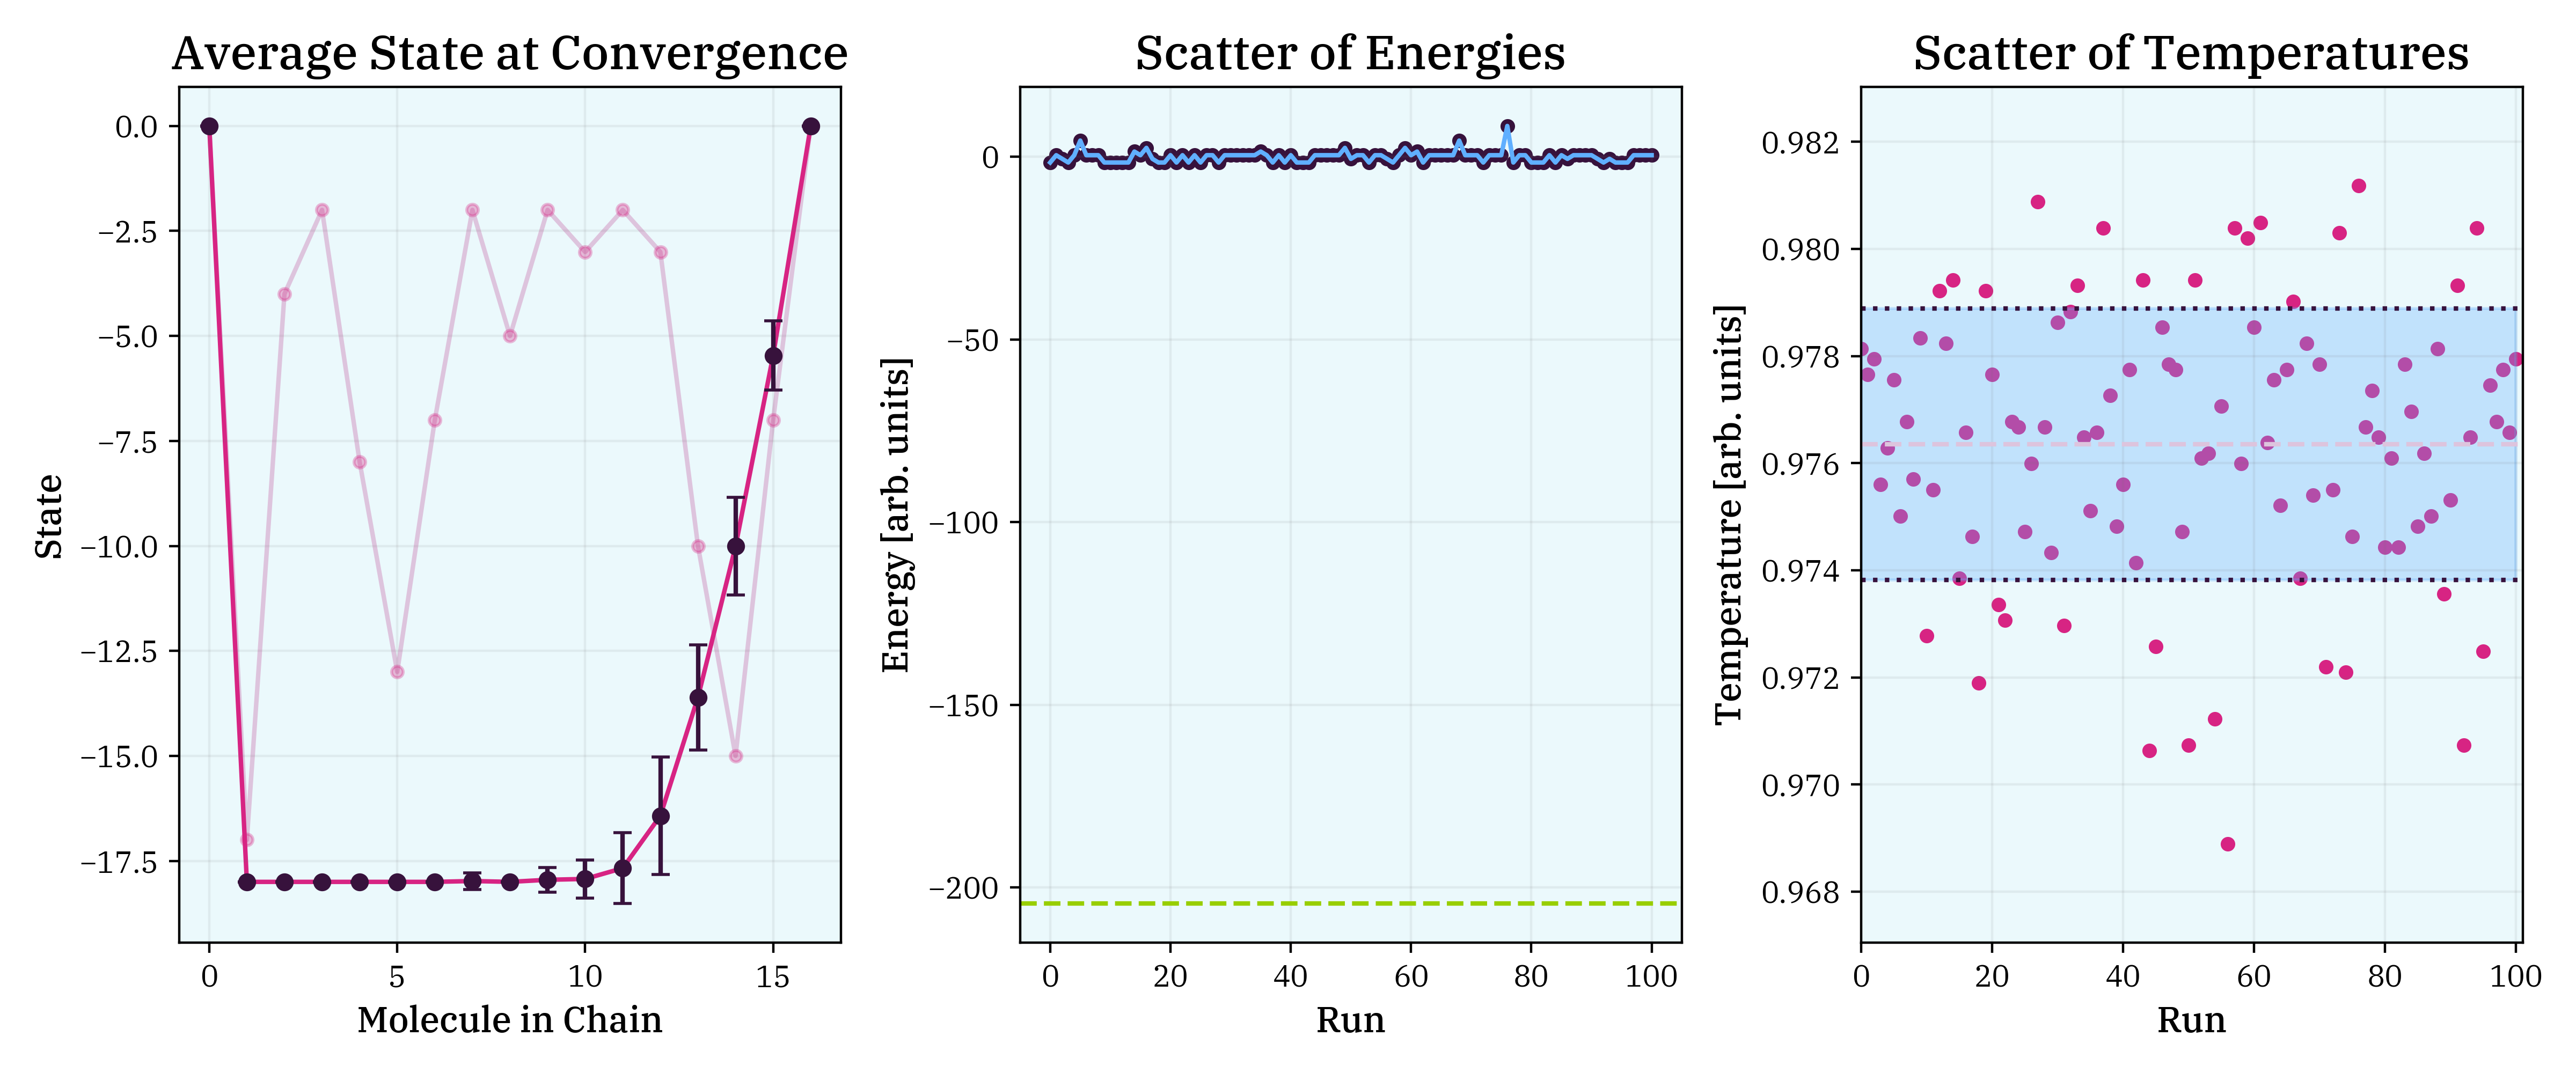
\includegraphics[width=.95\textwidth]{../fixed-init-multiple.png}
    \caption{Final state, Temperature, Energy scatter over runs for the molecular chain at a fixed initial state.}
    \label{fig:molecular-demo}
\end{figure}

It was here that I also experimented slightly with the parameters of the chain, such as length or allowed molecule depth.
For example I managed to find a state that optimized almost to a chain link but since one of the molecules was on the top level it tried to make 
two chain links, as displayed in Figure (\ref{fig:chain-link}). 

\begin{figure}[h!]
    \centering
    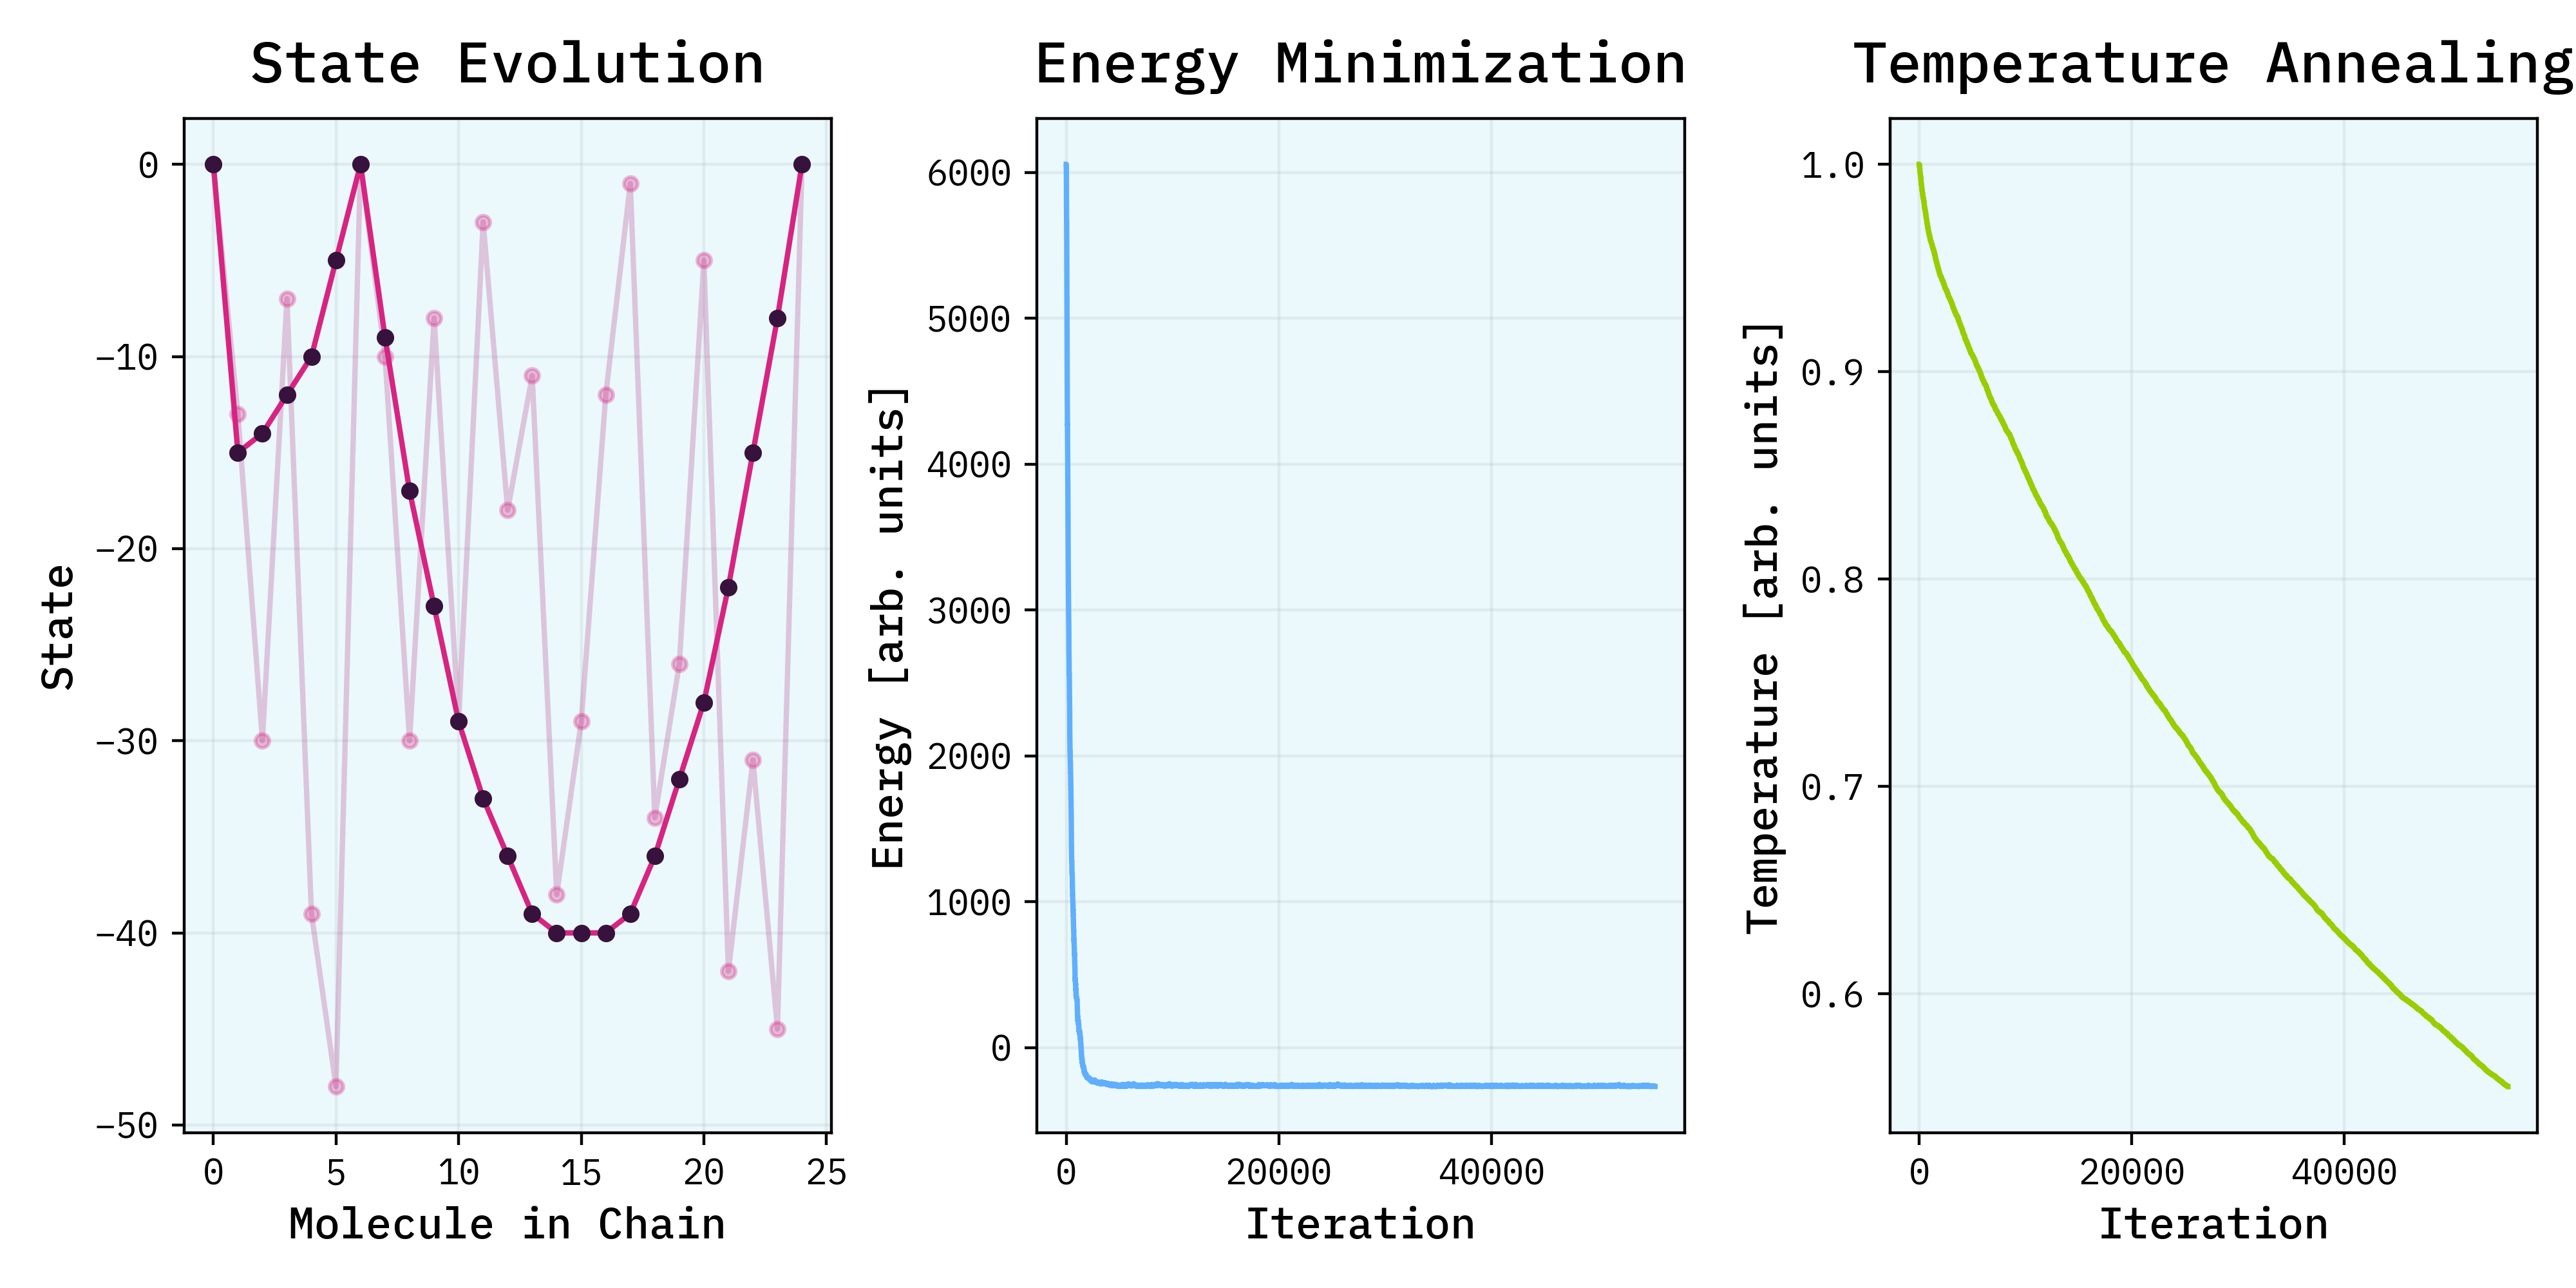
\includegraphics[width=.95\textwidth]{../accidental-veriznica.png}
    \caption{Optimized state of the molecular chain that almost forms a double chain link.}
    \label{fig:chain-link}
\end{figure}

I also trid maximize the \textit{curlyness} of the chain by modifiying the coefficients of the energy function. One of my better attempts is plotted 
in Figure (\ref{fig:curly-chain}), where the elastic energy term is set to be $10$ times larger.

\begin{figure}[H]
    \centering
    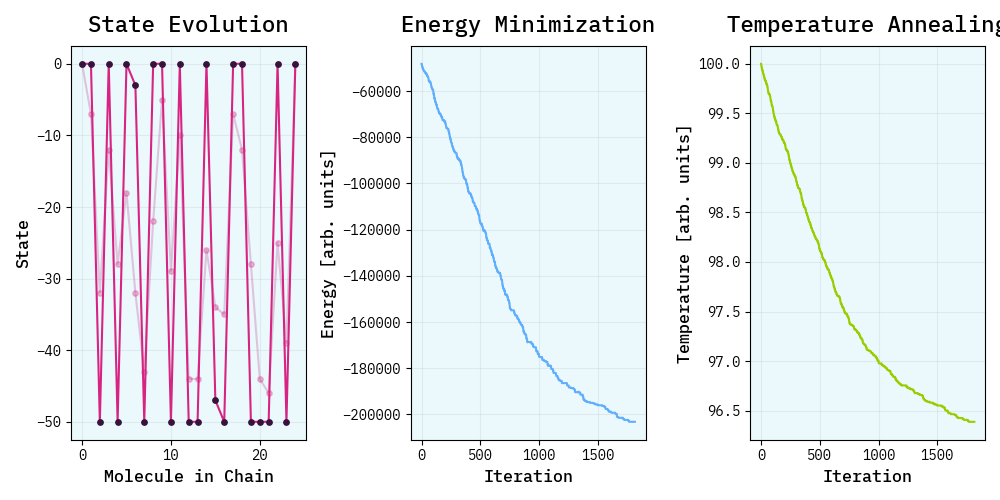
\includegraphics[width=.95\textwidth]{../curly-boi-Beta10.png}
    \caption{Optimized state of the molecular chain that is maximally curly.}
    \label{fig:curly-chain}
\end{figure}

The rest of the results for the molecular chain are displayed in the results section as I think they are more than just intermediate results or 
random observations.

\subsection{Ising Model}
After (re)writing the code for the molecular chain I adapted it for the Ising model, creating a solver class \texttt{Metropolis2}. I had a few problems
with the scale of energy and temperature but I think I managed to solve those in the end and the results seem to be reasonable. Data was also stored in 
a \texttt{HDF5} file, due to the sheer volume as I wanted a decent sample size for my statistics. The main challenge was the code being relatively slow 
per lattice and I wanted to simulate long times. As much as I promised not to focus on optimization I did to single-computer parallelization by utilizing
the \texttt{ProcessPoolExecutor} from the \texttt{concurrent.futures} module of Python. As stated above, a class-based approach allowed me to easily
spawn multiple instances of the solver class with different parameters on different processes which greatly sped up the gathering of data. I think this 
style of parallelization is reasonable as it takes very little time to implement and yields significant speedups. Here is 
a brief overview of how \texttt{ProcessPoolExecutor} is used:

\lstinputlisting[language=Python]{code-demo.txt}

I have to mention somewhere that I accidentally kept Simulated Annealing on for some of the temperature dependance studies, which meant 
I had to recalculate a lot of data. Anyways, let's get to some images. Like before some debug style plots at the beginning definitely do not 
hurt. I wanted to get a feel for where the critical temperature is and how long it takes to reach equilibrium. For the purpose of 
nicer images I ran the simulation for a $500\times 500$ lattice, as the professor commented that this size would give nice-looking 
results. Figure (\ref{fig:ising-demo-subcritical}) shows the initial and final states of the lattice at a subcritical temperature of $T=1$.

\begin{figure}[H]
    \centering
    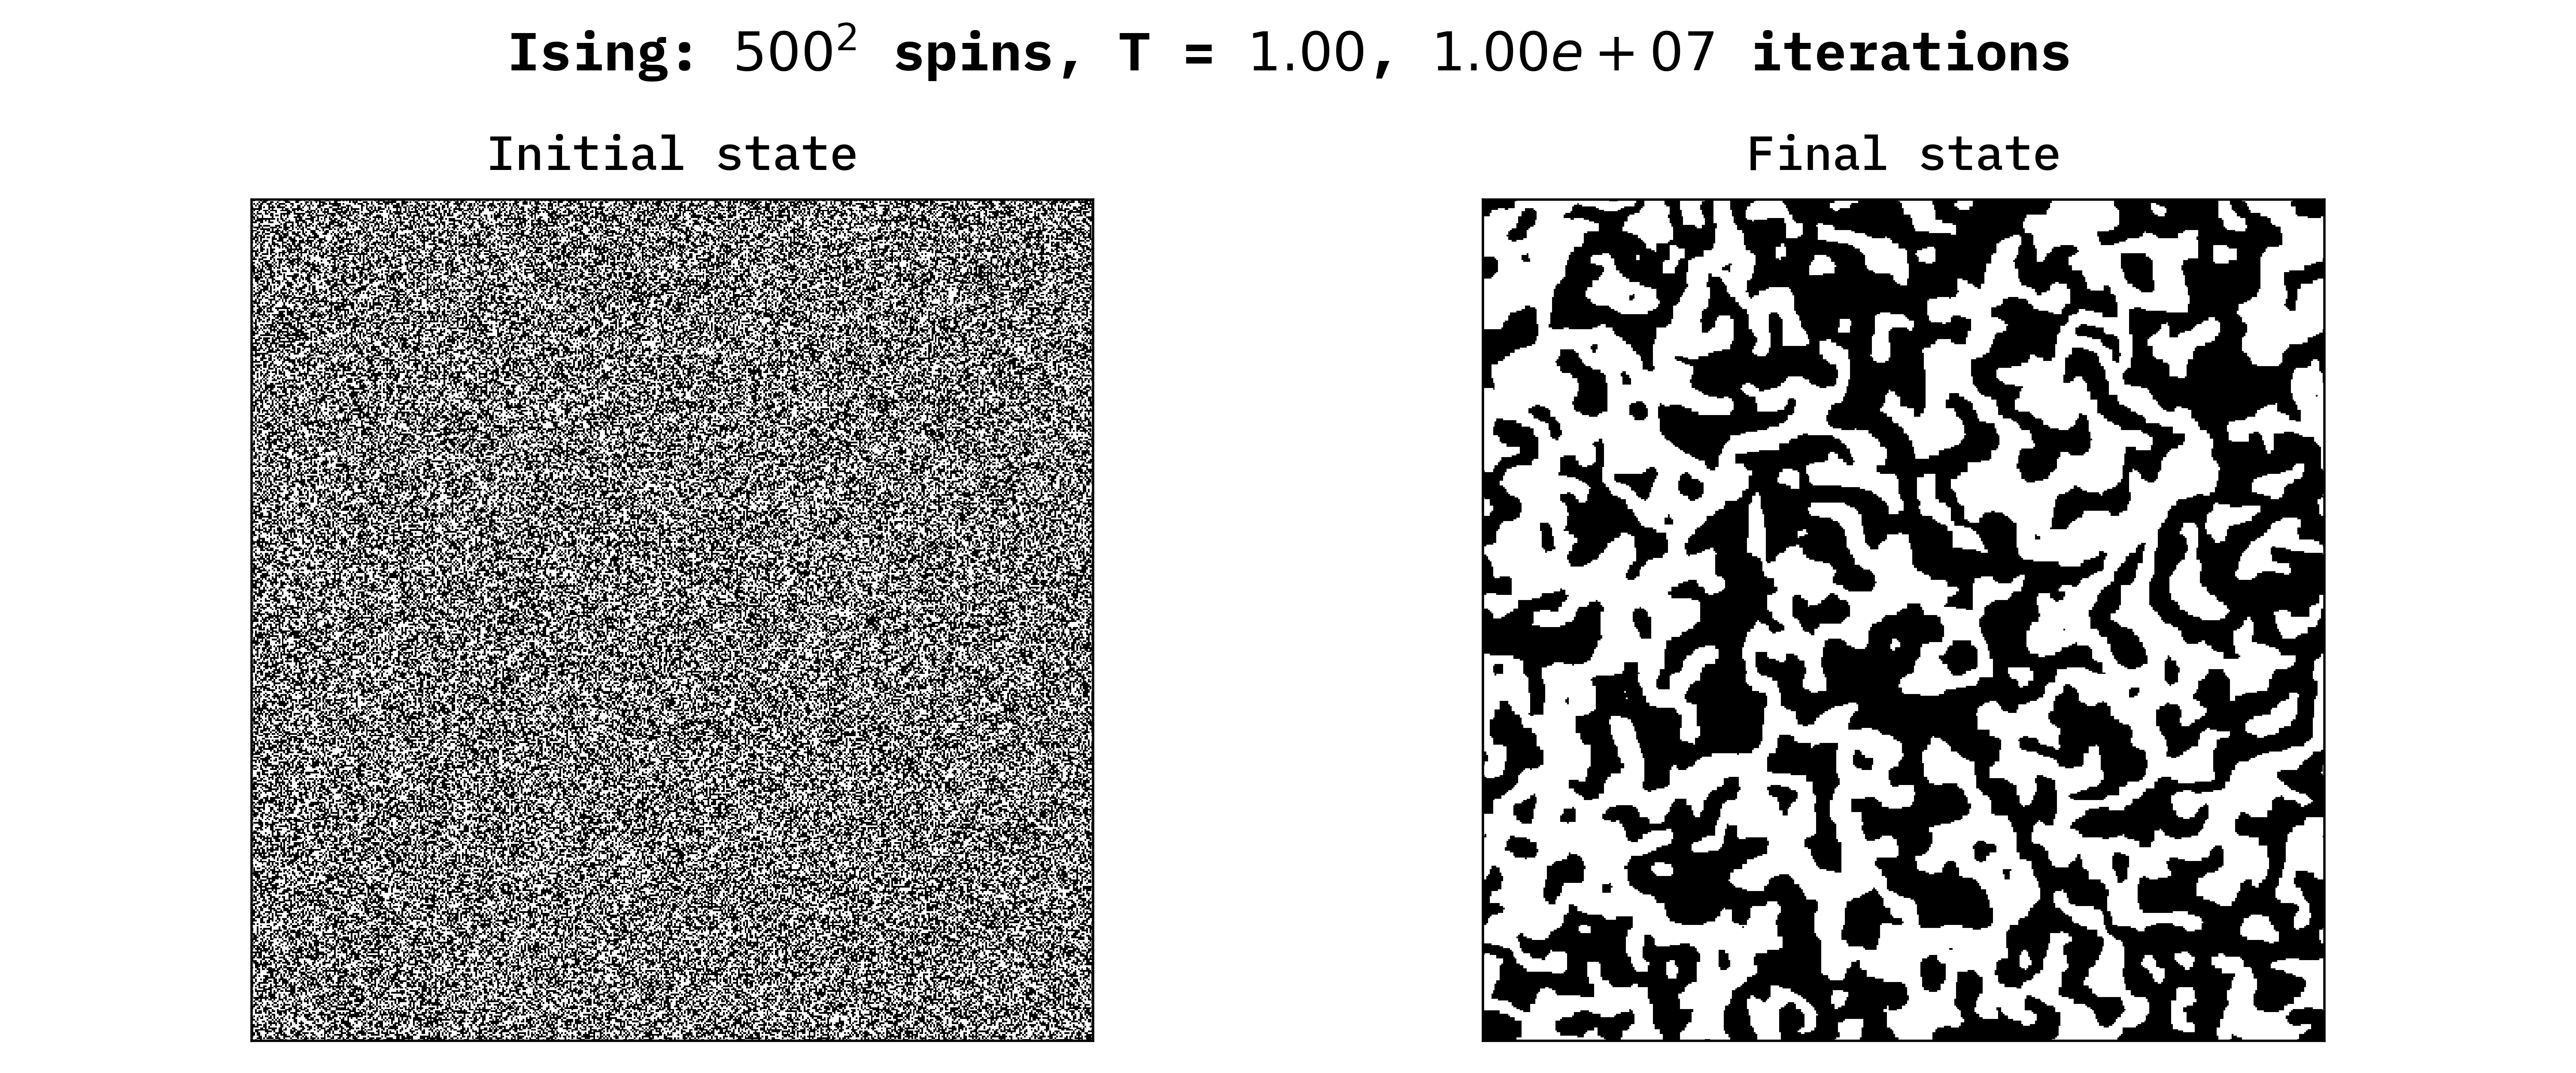
\includegraphics[width=.95\textwidth]{../IsingModel/Images/ising-demo-subcritical.png}
    \caption{Initial and final states of the Ising model lattice at a subcritical temperature of $T=1$.}
    \label{fig:ising-demo-subcritical}
\end{figure}

We can see that the lattice is in a ferromagnetic state and that magnetic domains have nicely formed. The lattice is drastically different 
from the initial state. It now only makes sense to take a look at a supercritical temperature of $T=10$ which is displayed 
in Figure (\ref{fig:ising-demo-supercritical}).

\begin{figure}[H]
    \centering
    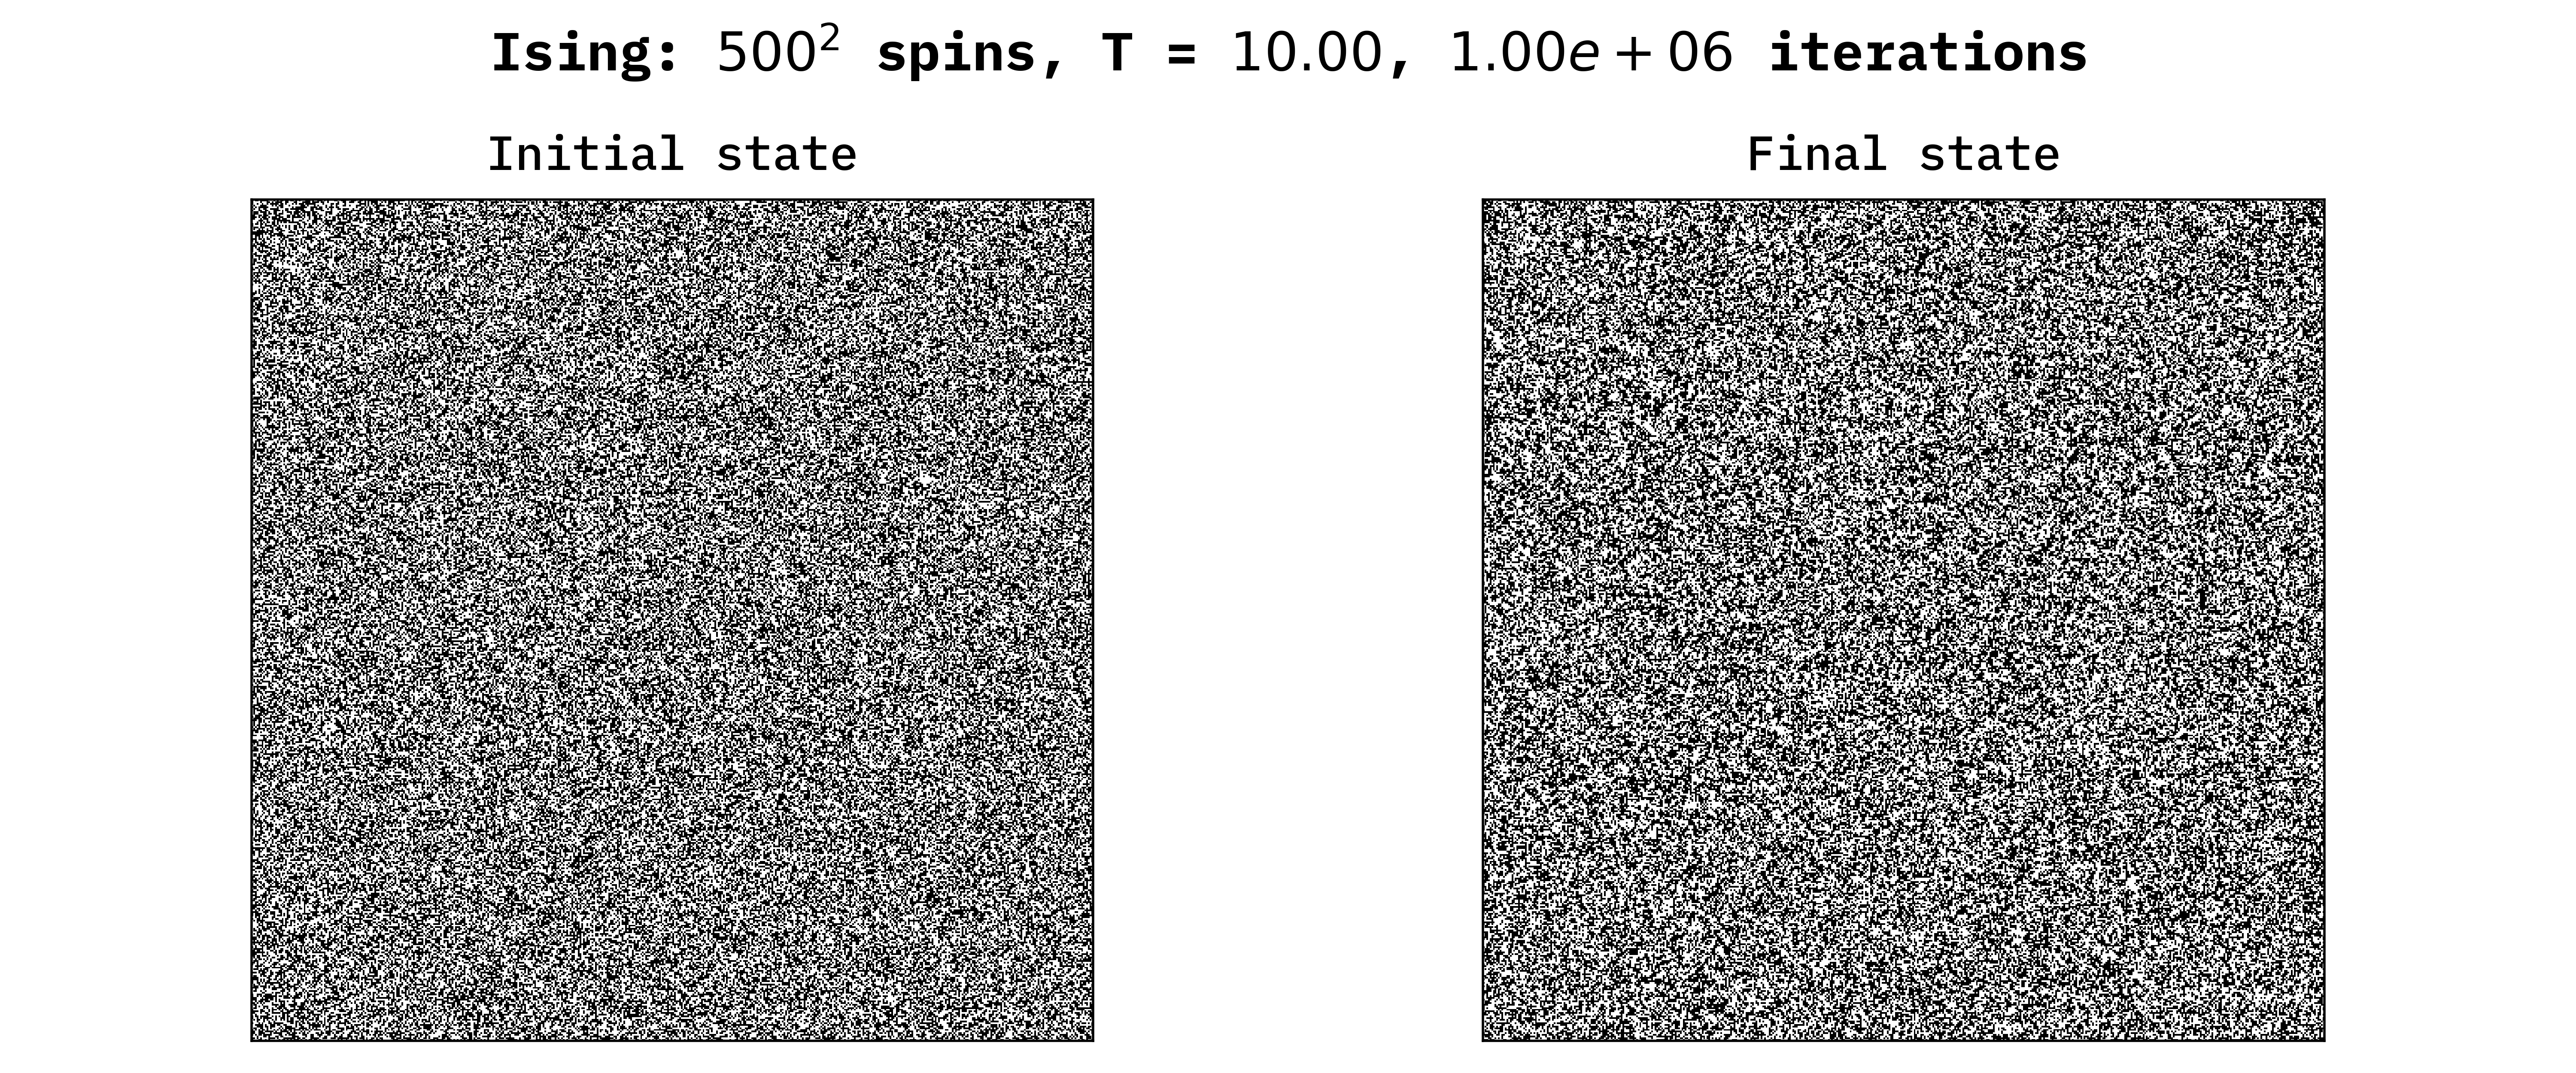
\includegraphics[width=.95\textwidth]{../IsingModel/Images/ising-demo-supercritical.png}
    \caption{Initial and final states of the Ising model lattice at a supercritical temperature of $T=10$.}
    \label{fig:ising-demo-supercritical}
\end{figure}

The lattice looks very simmilar to the initial state which is expected as we do not expect spontaneous magnetization at supercritical temperatures.
I was also interested in how the lattice behaves at the critical temperature, which is forcasted by the Onsager solution (\ref{eq:onsager}) to be
$T_c\approx 2.269185$. The result is displayed in Figure (\ref{fig:ising-demo-critical}).

\begin{figure}[H]
    \centering
    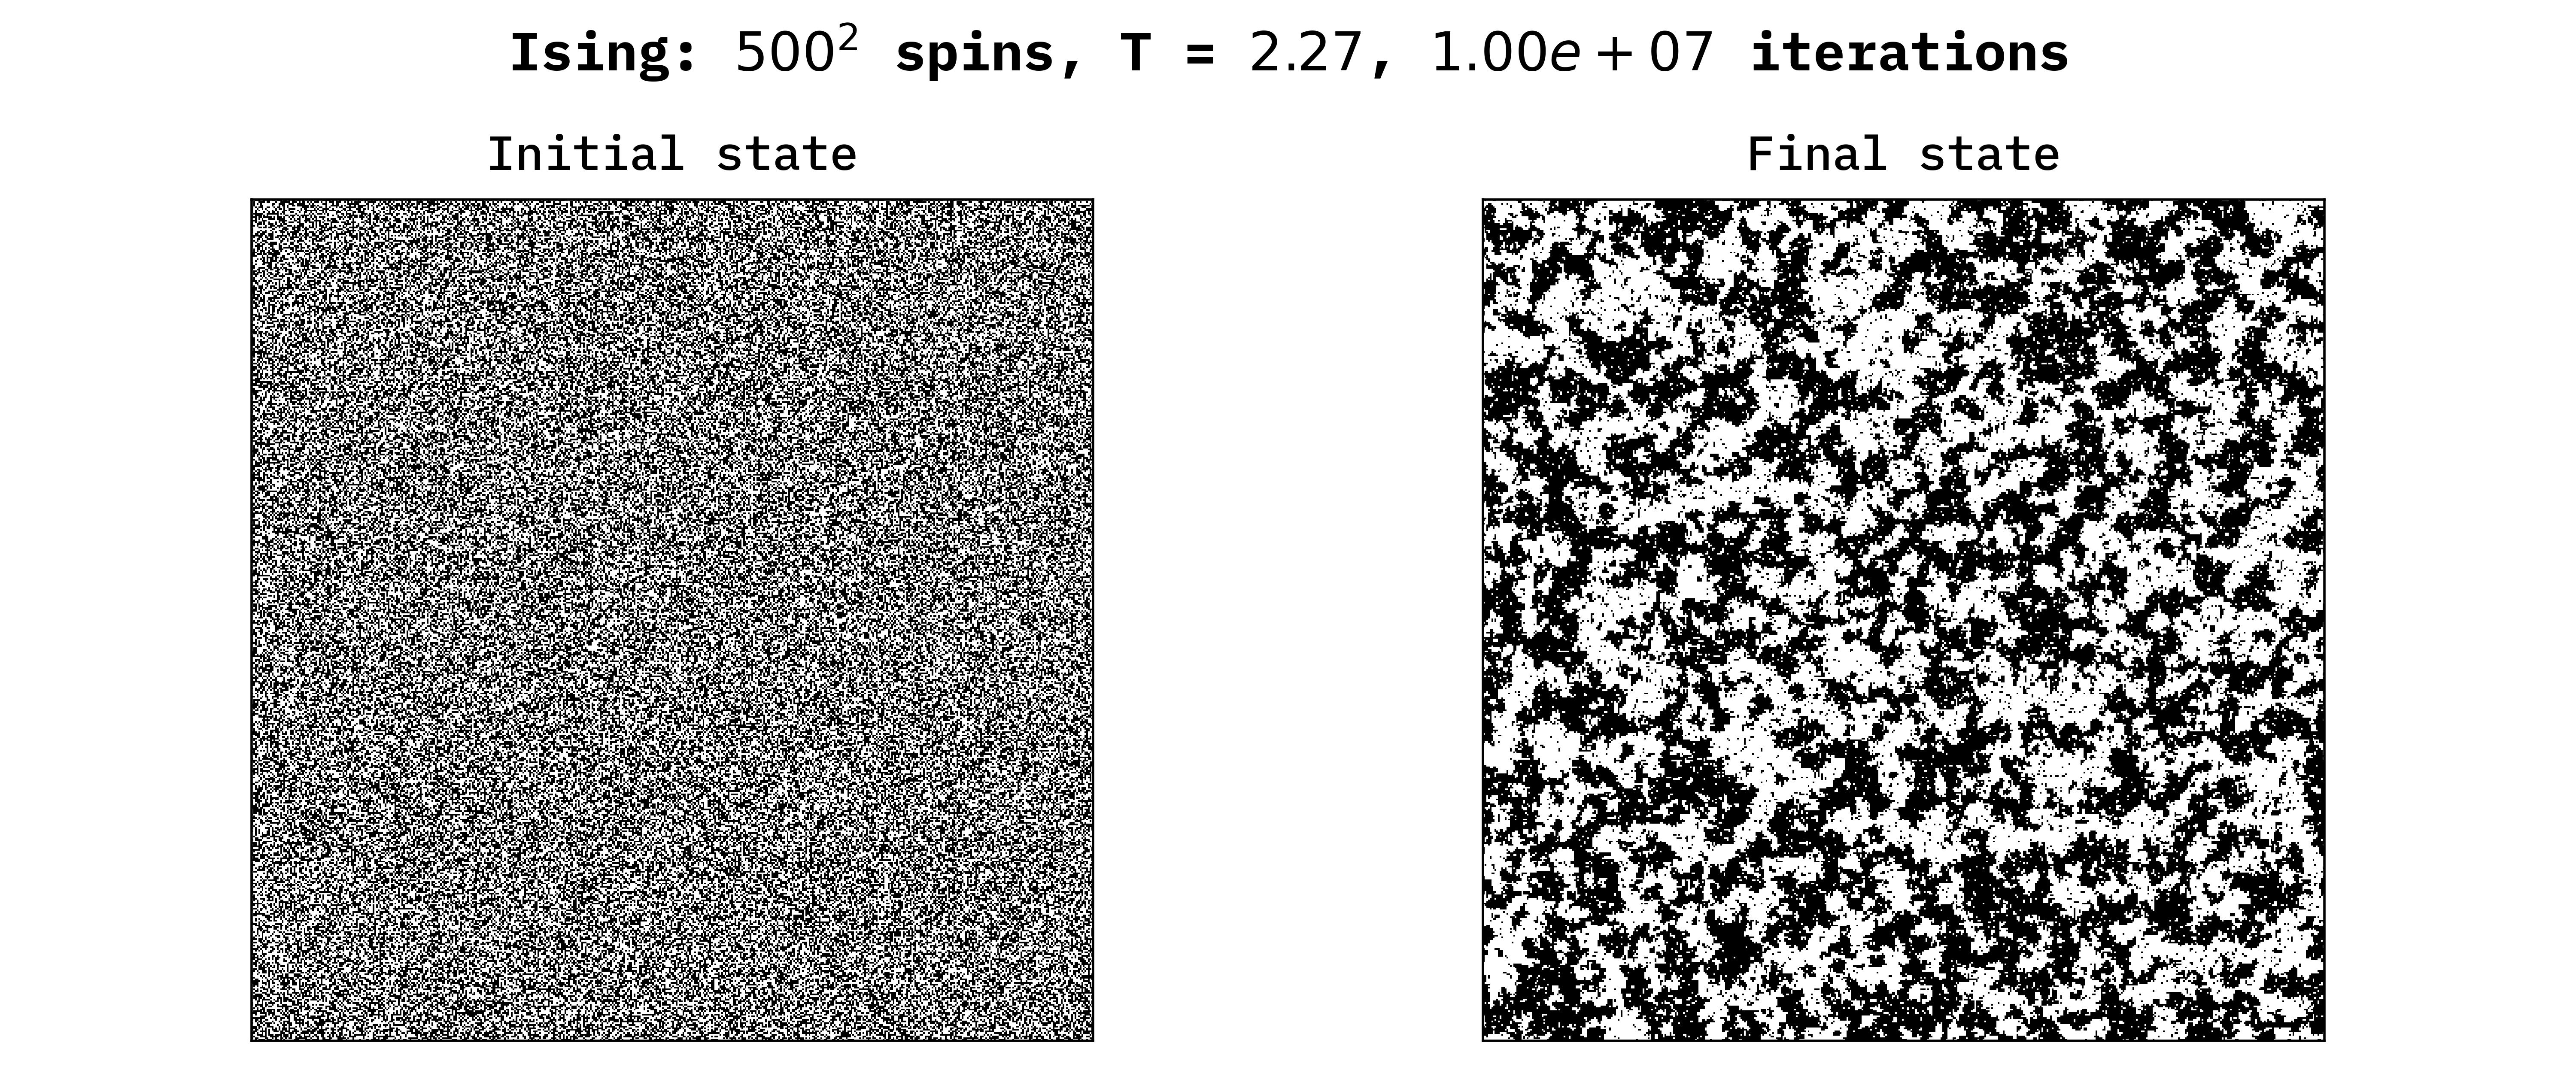
\includegraphics[width=.95\textwidth]{../IsingModel/Images/ising-demo-critical.png}
    \caption{Initial and final states of the Ising model lattice at the critical temperature of $T\approx 2.269185$.}
    \label{fig:ising-demo-critical}
\end{figure}

The lattice is sort of a mix between the subcritical and supercritical states, which is exactly what we expect. Visually it looks like a grainyer
version of the ferromagnetic state. As a final little debug plot I wanted to see what a state would look like if I allowed more than just 
$|\ua\ra$ and $|\da\ra$ states. As an attempt at a generalization to $s=3/2$ particles I allowed for states to go from $-2$ to $2$. The result of 
optimizing such a lattice with the same Hamiltonian at a subcritical temperature is displayed in Figure (\ref{fig:ising-demo-3/2-subcrit}).

\begin{figure}[H]
    \centering
    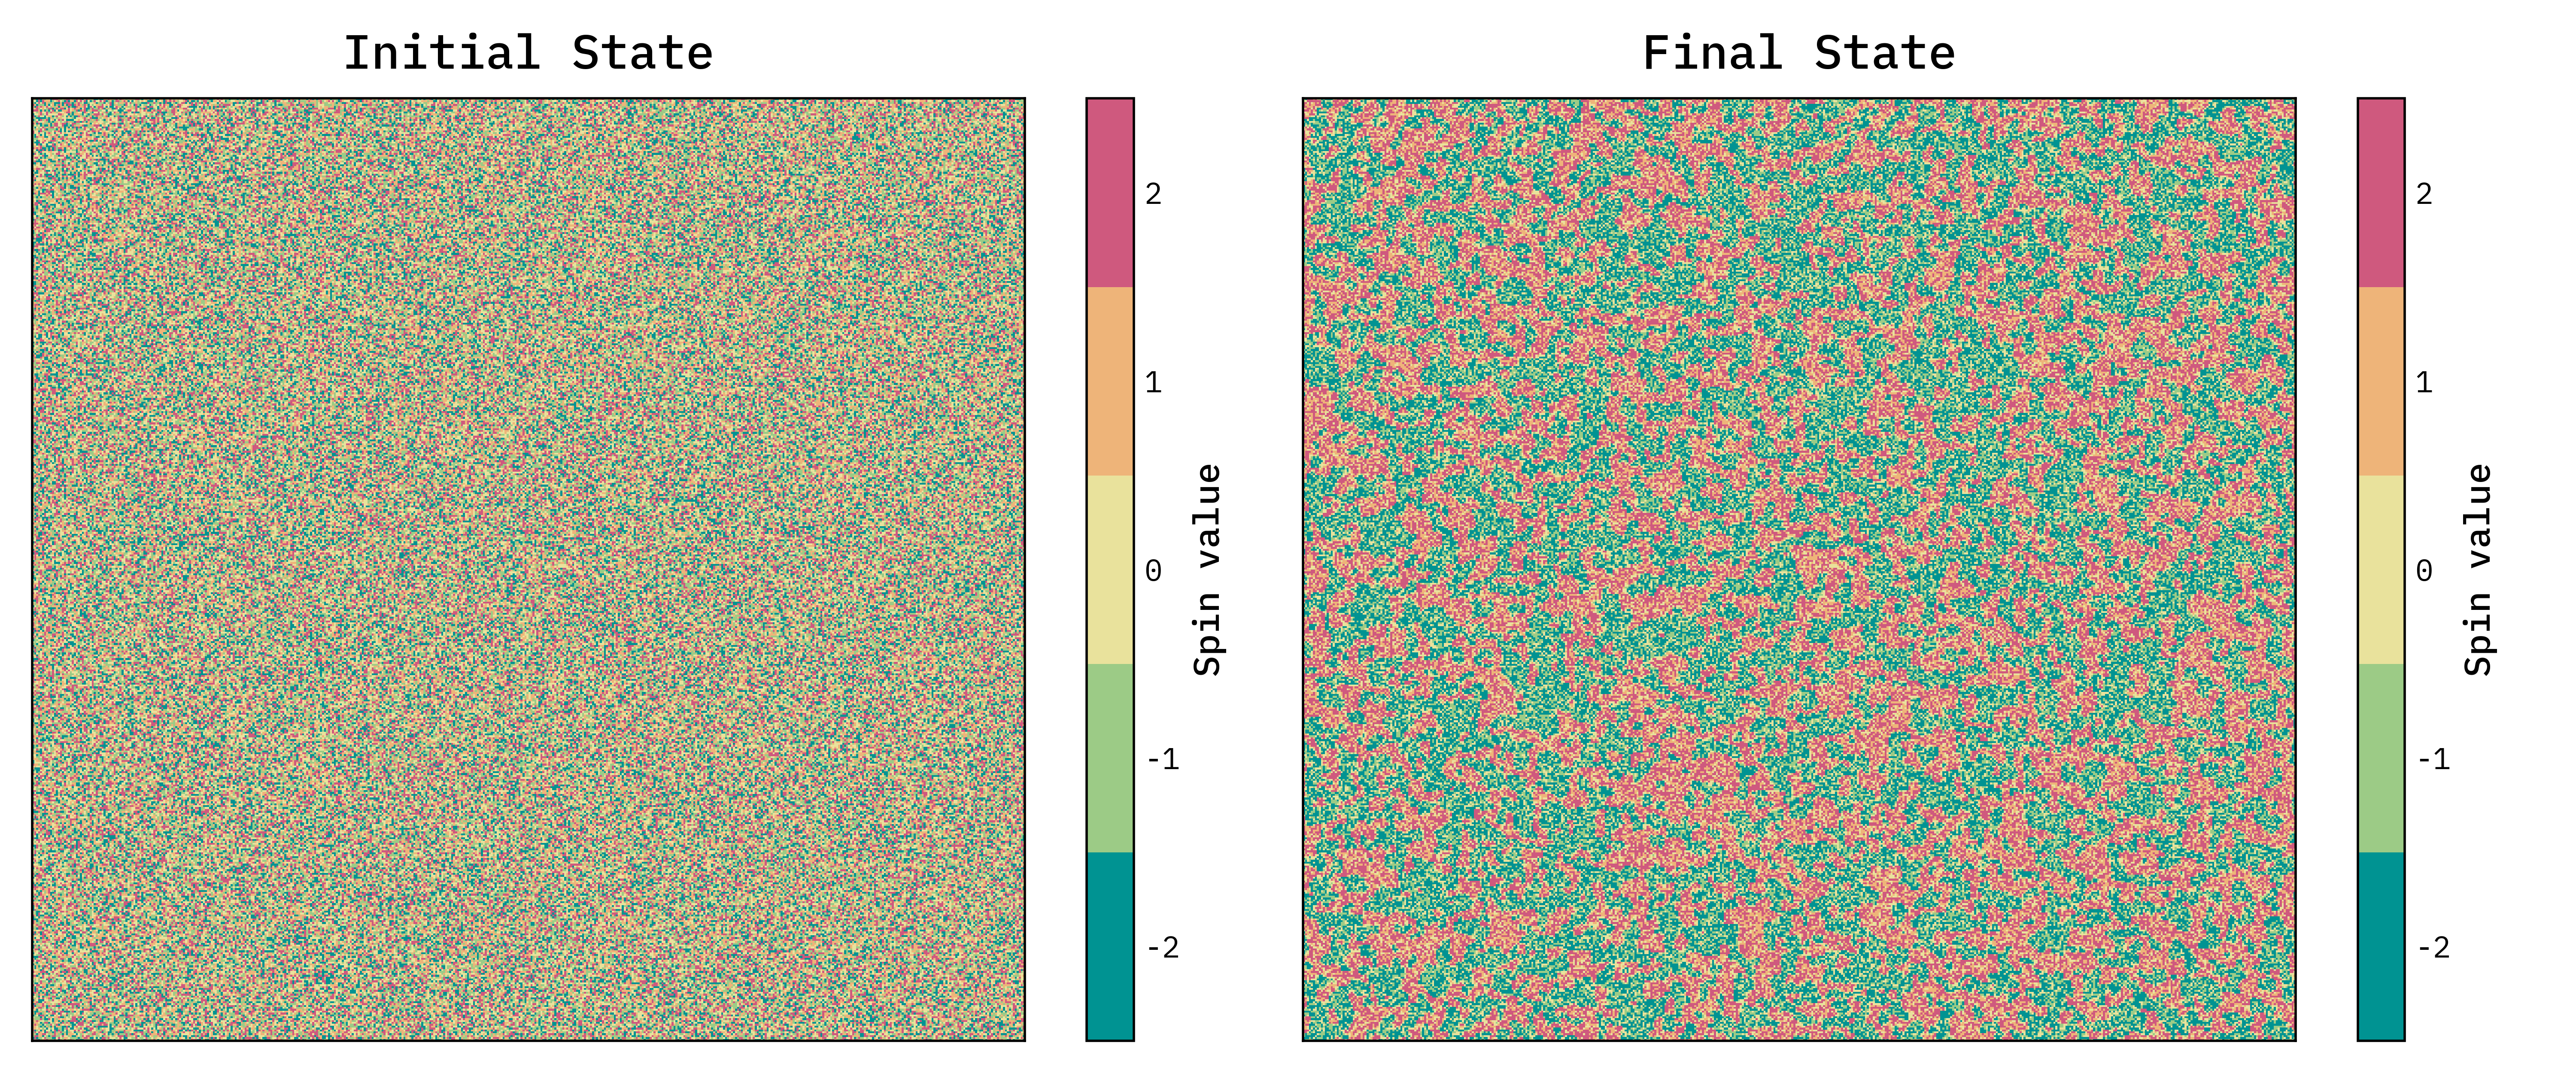
\includegraphics[width=.95\textwidth]{../IsingModel/Images/expanded-state-subcritical.png}
    \caption{Initial and final states of the Ising model lattice with $s=3/2$ particles at a subcritical temperature of $T=1$.}
    \label{fig:ising-demo-3/2-subcrit}
\end{figure}

The lattice looks very similar to the $s=1/2$ lattice however with more variation. I find it interesting that patches of states $2$ and $-2$ 
surround themselves with states $1$ and $-1$. I have no idea if this model has any real life applications however. I wish I had enough time to 
explore this further. Analogous to $s=1/2$ particles we can expect interesting behavior at the critical temperature. The result is displayed in
Figure (\ref{fig:ising-demo-3/2-critical}).

\begin{figure}[H]
    \centering
    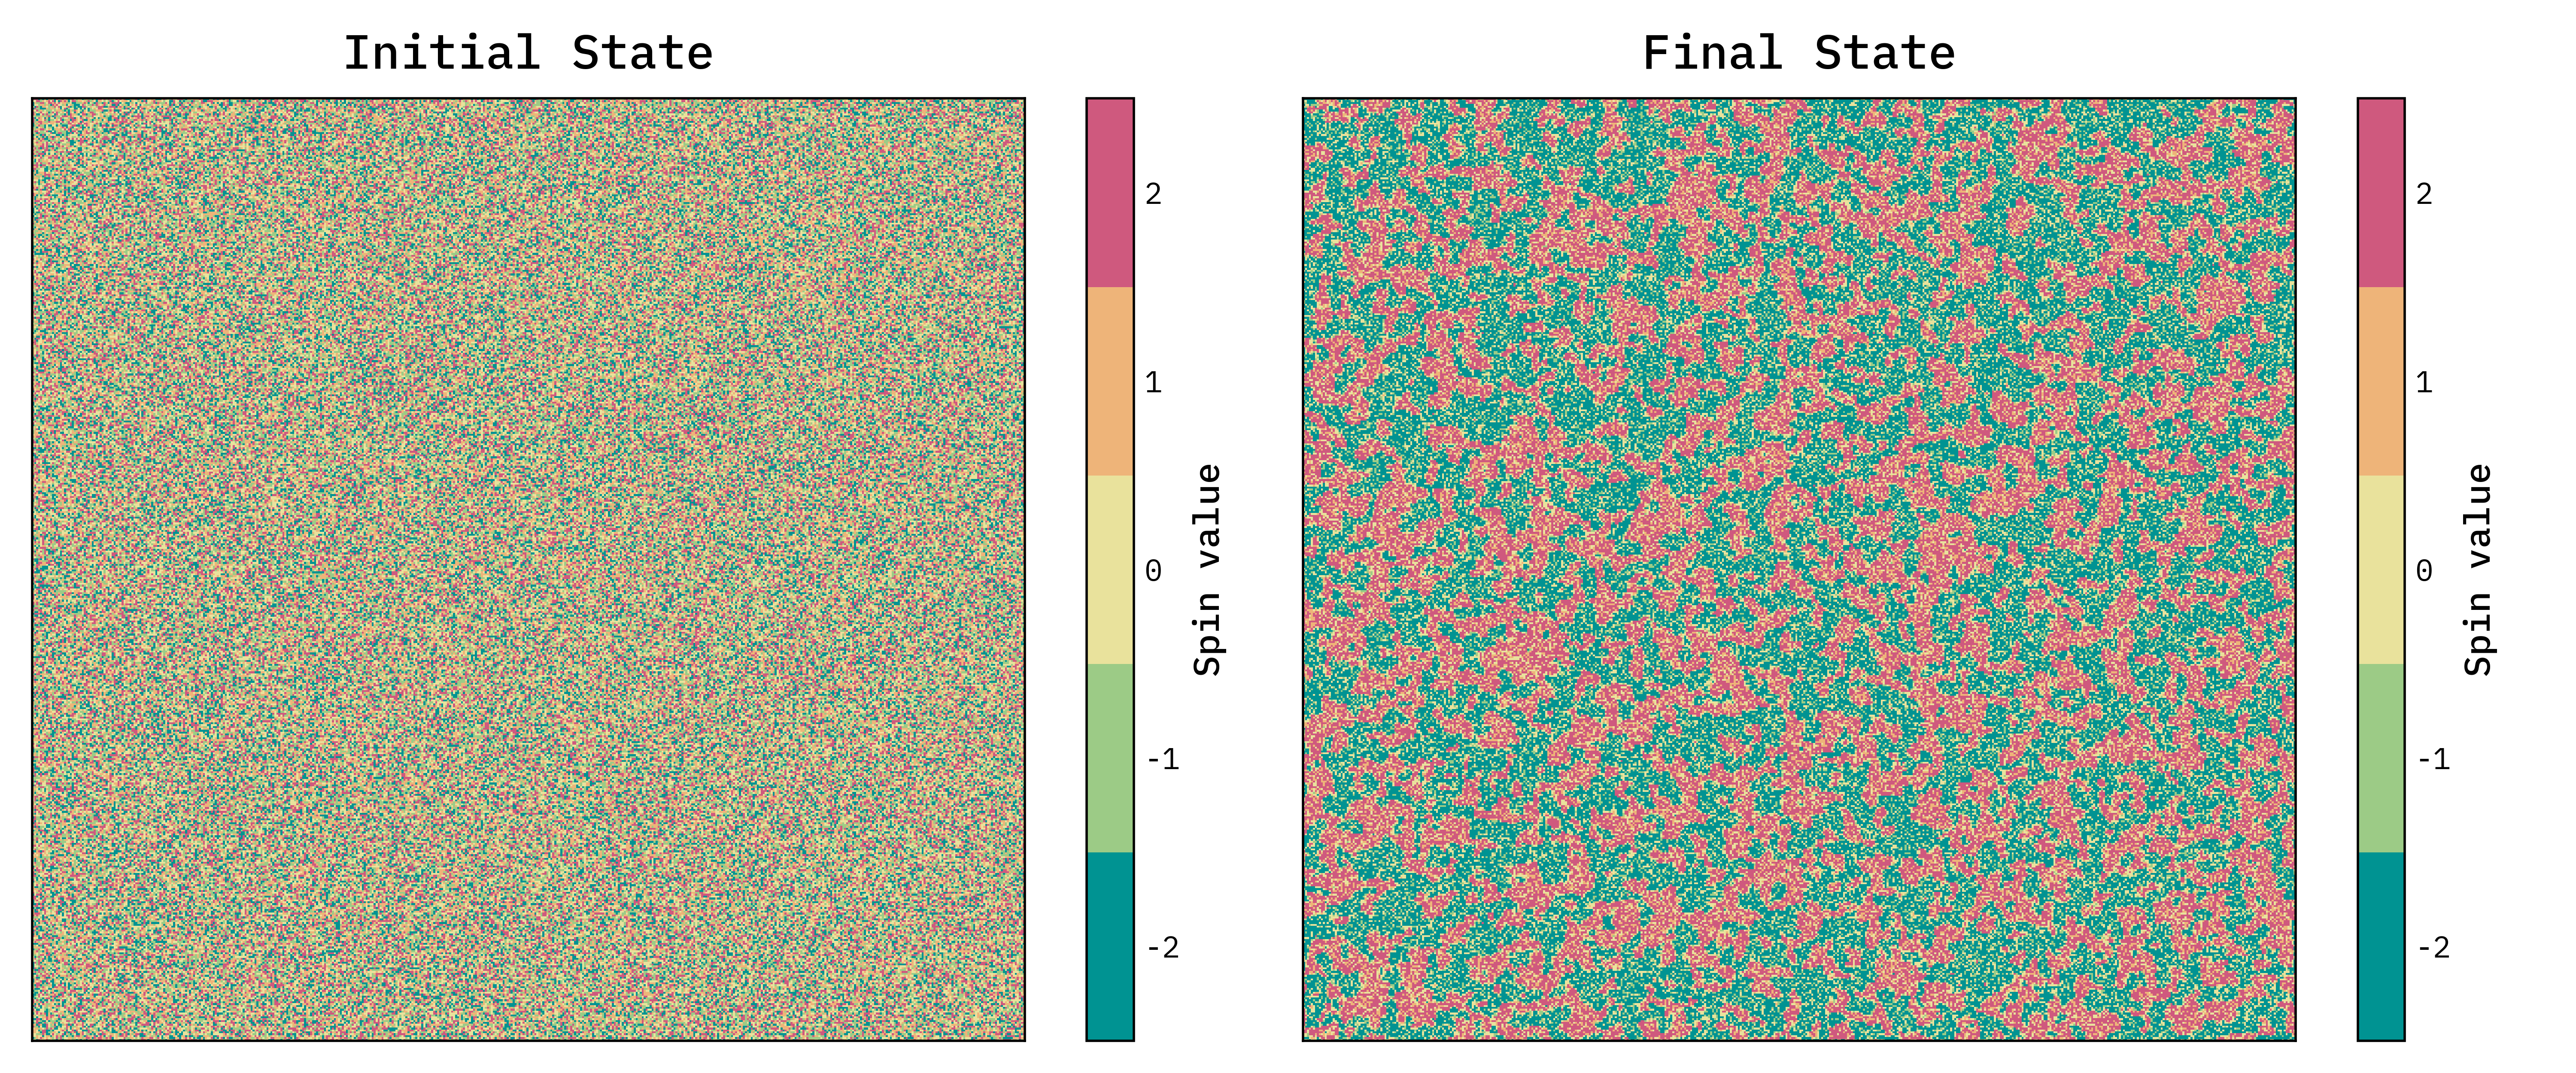
\includegraphics[width=.95\textwidth]{../IsingModel/Images/expanded-state-critical.png}
    \caption{Initial and final states of the Ising model lattice with $s=3/2$ particles at the critical temperature of $T\approx 2.27$.}
    \label{fig:ising-demo-3/2-critical}
\end{figure}

I'm not going to lie, the results look very simmilar to the subcritical temperature lattice with $s=3/2$ particles. Maybe even less \textit{dusty}
which is odd because I would expect the opposite. Due to a lack of time I did not have the liberty of exploring this further by, for example, gathering
more data and doing a statistical analysis instead of eesentialy an empirical one. For completeness I also ran the simulation at a supercritical
temperature of $T=10$ which is displayed in Figure (\ref{fig:ising-demo-3/2-supercrit}) where we get exactly what we expect, random noise more or less.
Although it does appear somewhat more structured.

\begin{figure}[H]
    \centering
    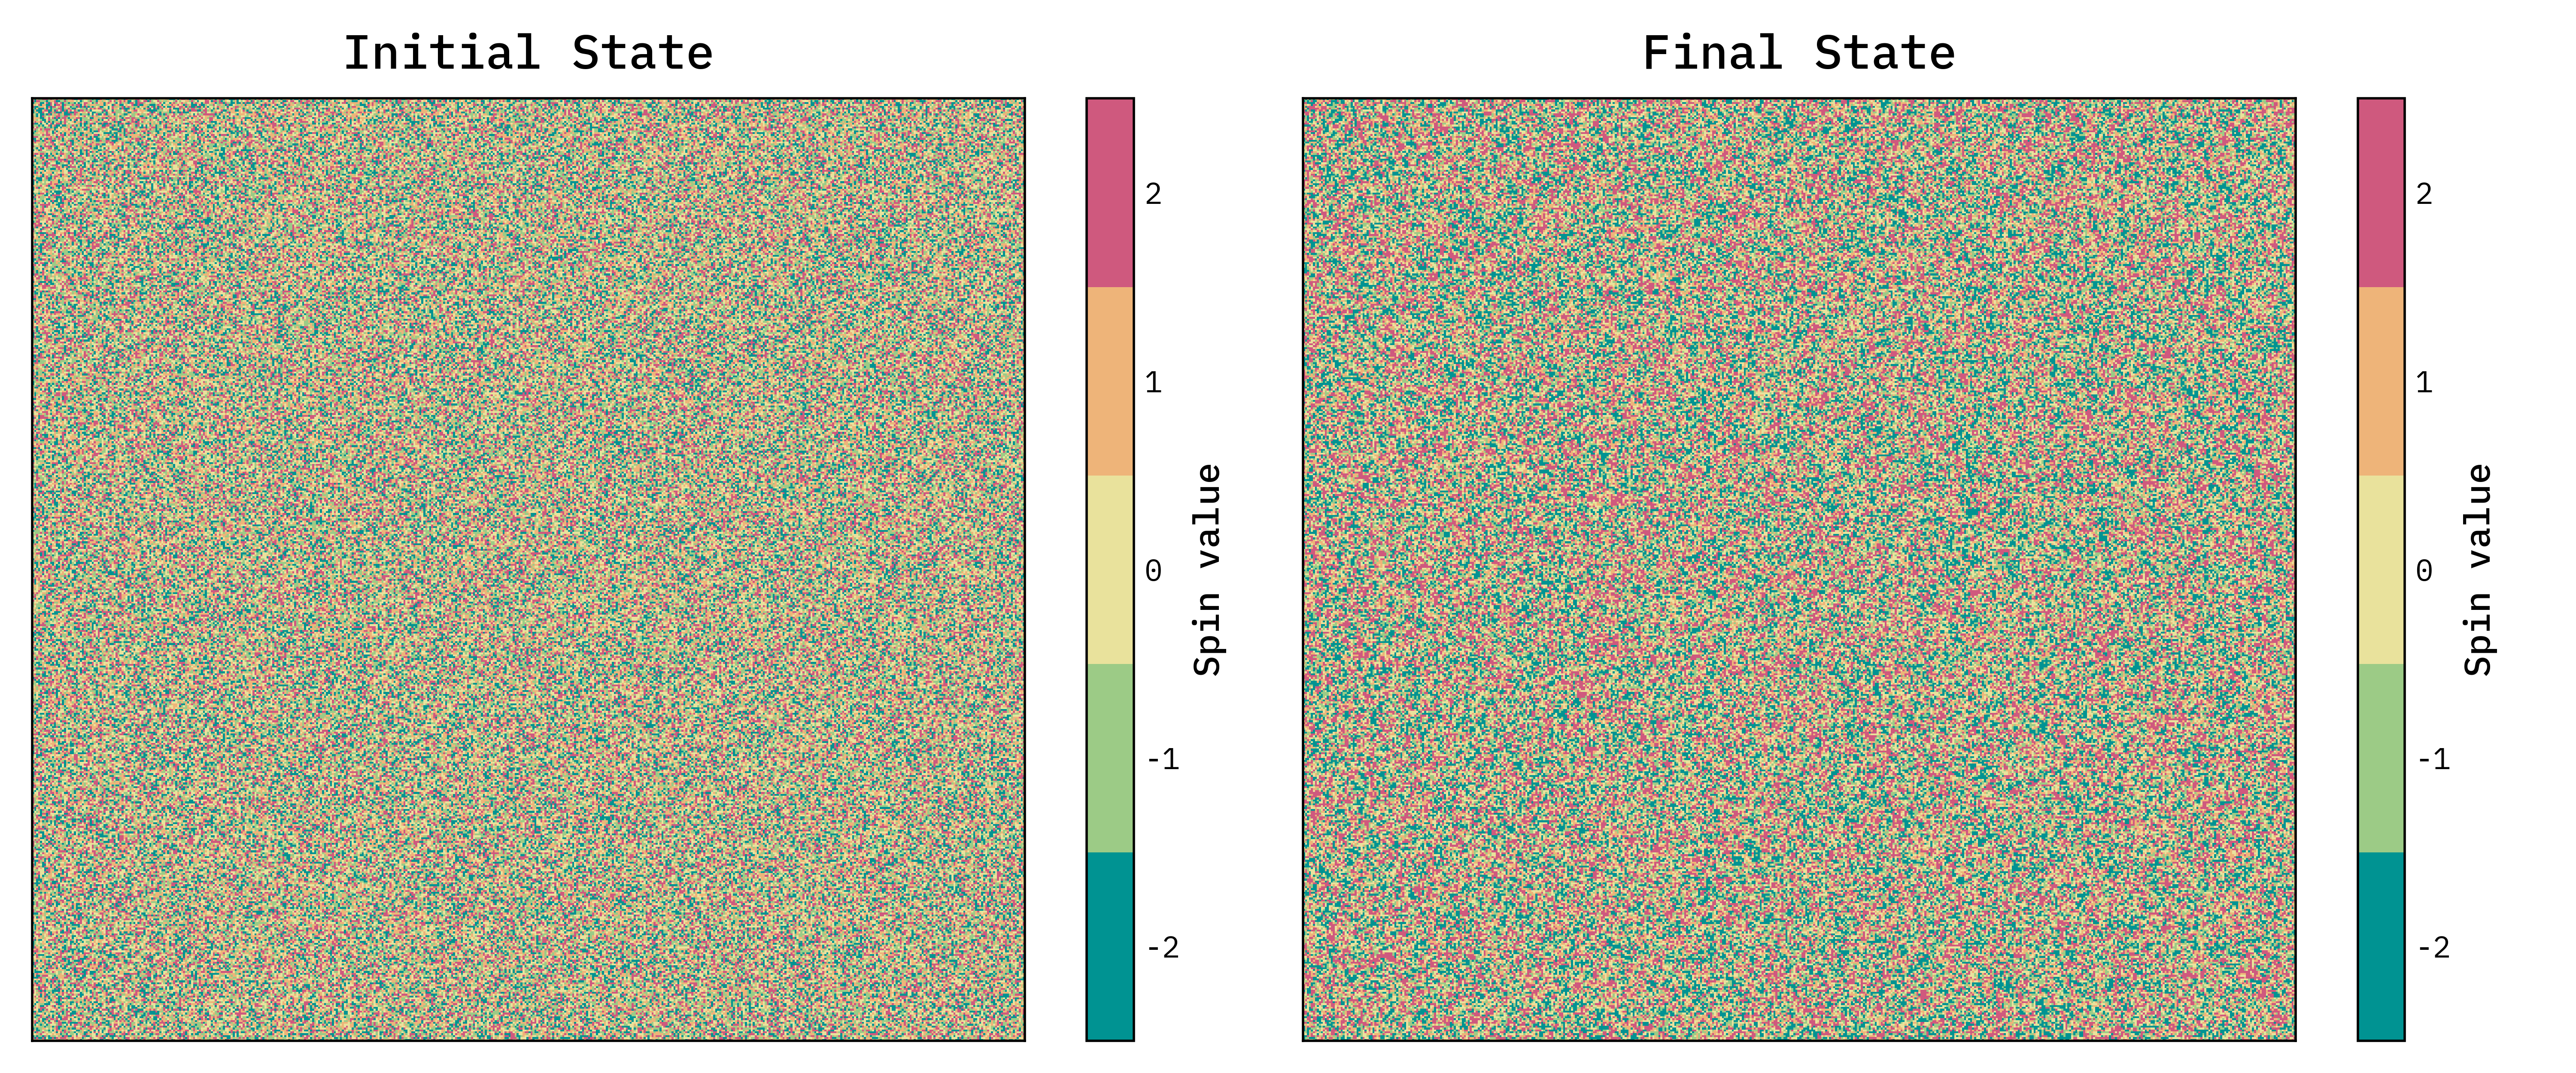
\includegraphics[width=.95\textwidth]{../IsingModel/Images/expanded-state-supercritical.png}
    \caption{Initial and final states of the Ising model lattice with $s=3/2$ particles at a supercritical temperature of $T=10$.}
    \label{fig:ising-demo-3/2-supercrit}
\end{figure}

The rest of the relevant plots for the Ising model are displayed in the results section.

\section{Results}
\subsection{Molecular Chain}
The instructions of the task demanded that we explore the temperature dependance of the equilibrium energy, which is presented in Figure 
(\ref{fig:molecular-energy}). For better statistics due to the stochastic nature of the Metropolis-Hastings algorithm I ran the simulation
$100$ times for each temperature. This resulted in $10000$ data sets of multiple thousand points each, hence the need for \texttt{HDF5} storage.
As we can see from the image the equilibrium energy of the molecular chain decreases with temperature as is expected. The standard deviation 
of the energy also somewhat decreases with temperature, which is likewise to be expected. I thought it would be interesting to also see how many 
steps of the Metropolis algorithm were needed to reach my convergence criteria which was an $\varepsilon$ tolerance of $10^{-14}$ averaged out 
over the last $50$ steps. Below are also spreads of the final temperature and energy across the runs. I thought it was a neat alternative way 
to visually display the scatter of the data for each temperature.

\begin{figure}[H]
    \centering
    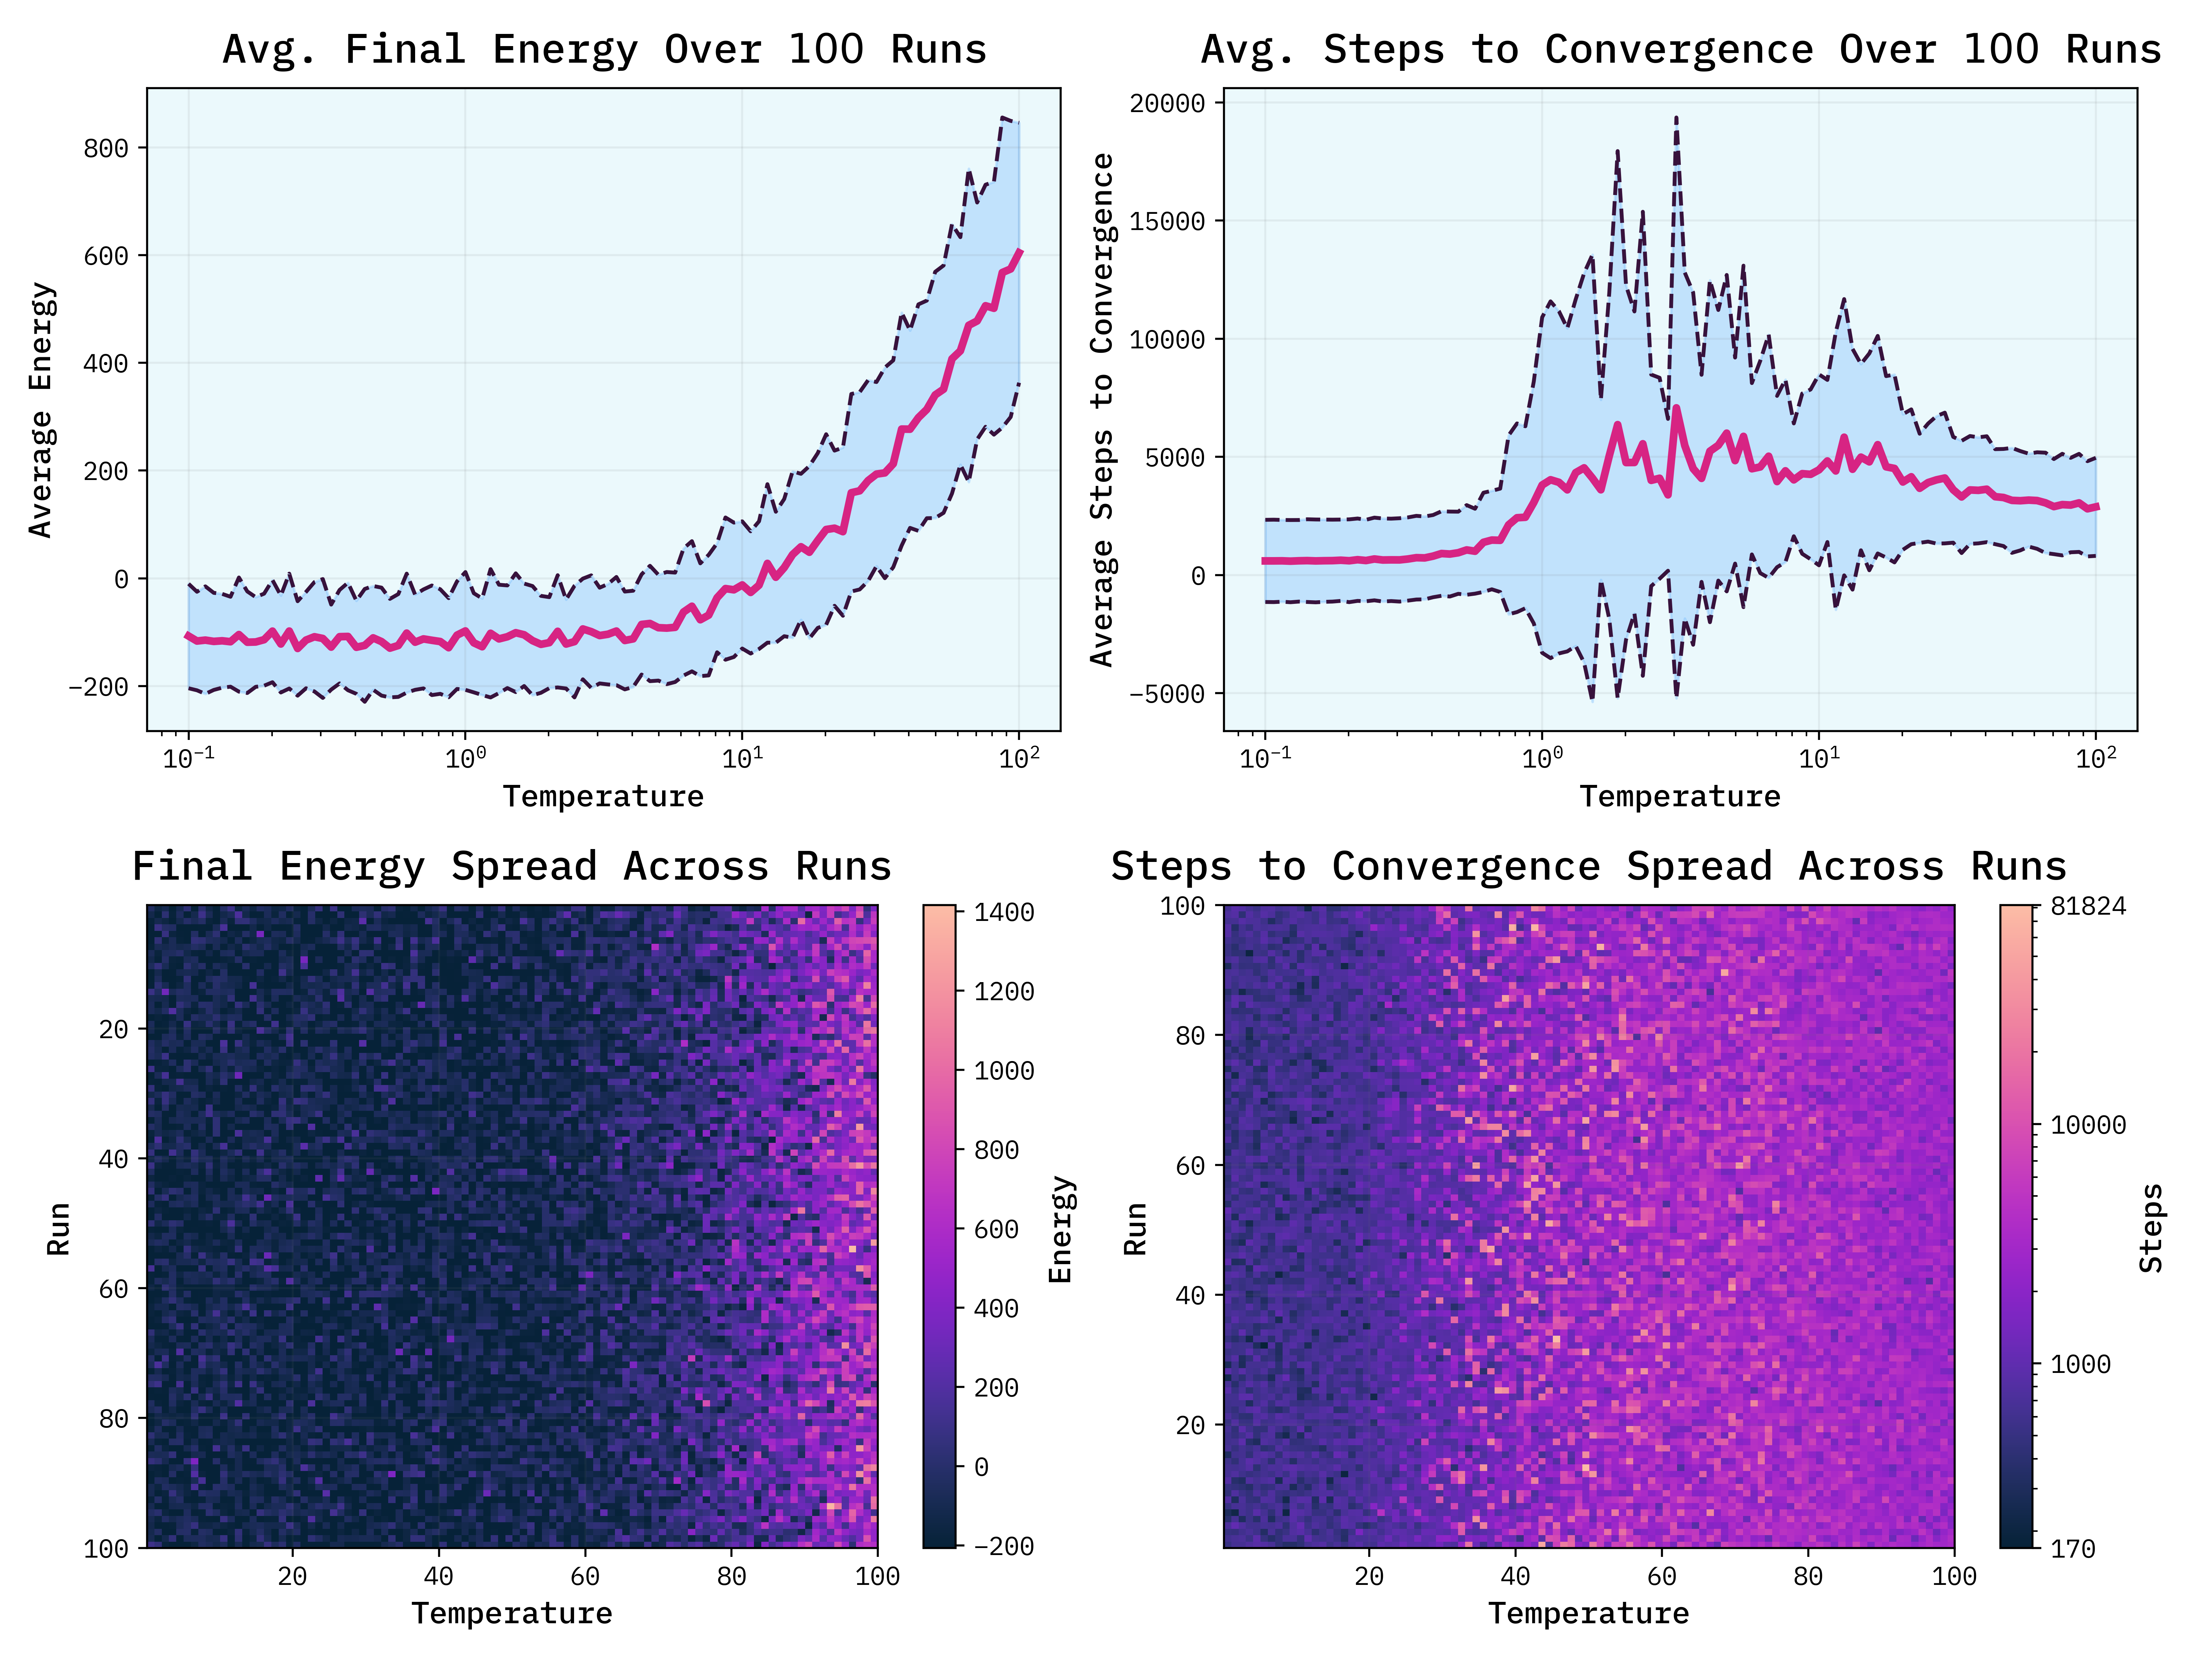
\includegraphics[width=.95\textwidth]{../MolecularChain2/Images/avgE-vs-T.png}
    \caption{Equilibrium energy of the molecular chain as a function of temperature.}
    \label{fig:molecular-energy}
\end{figure}

Since I had the data already gathered it was very simple to plot the average shape of the molecular chain across all temperatures. I also tried to 
display the average shapes over repeat runs for each temperature. The results are displayed in Figure (\ref{fig:molecular-chain-shapes}). It is 
interesting to note albeit expected that the shape optimizes best at medium to low temperatures. At high temperatures the chain can 
still jump around a lot and at low temperatures it can get stuck in local minima. Overall though we get quite a well defined shape that is close 
to the optimal. I find it insteresting that the left portion of the chain is always well defined while the right position has some uncertainty.

\begin{figure}[H]
    \centering
    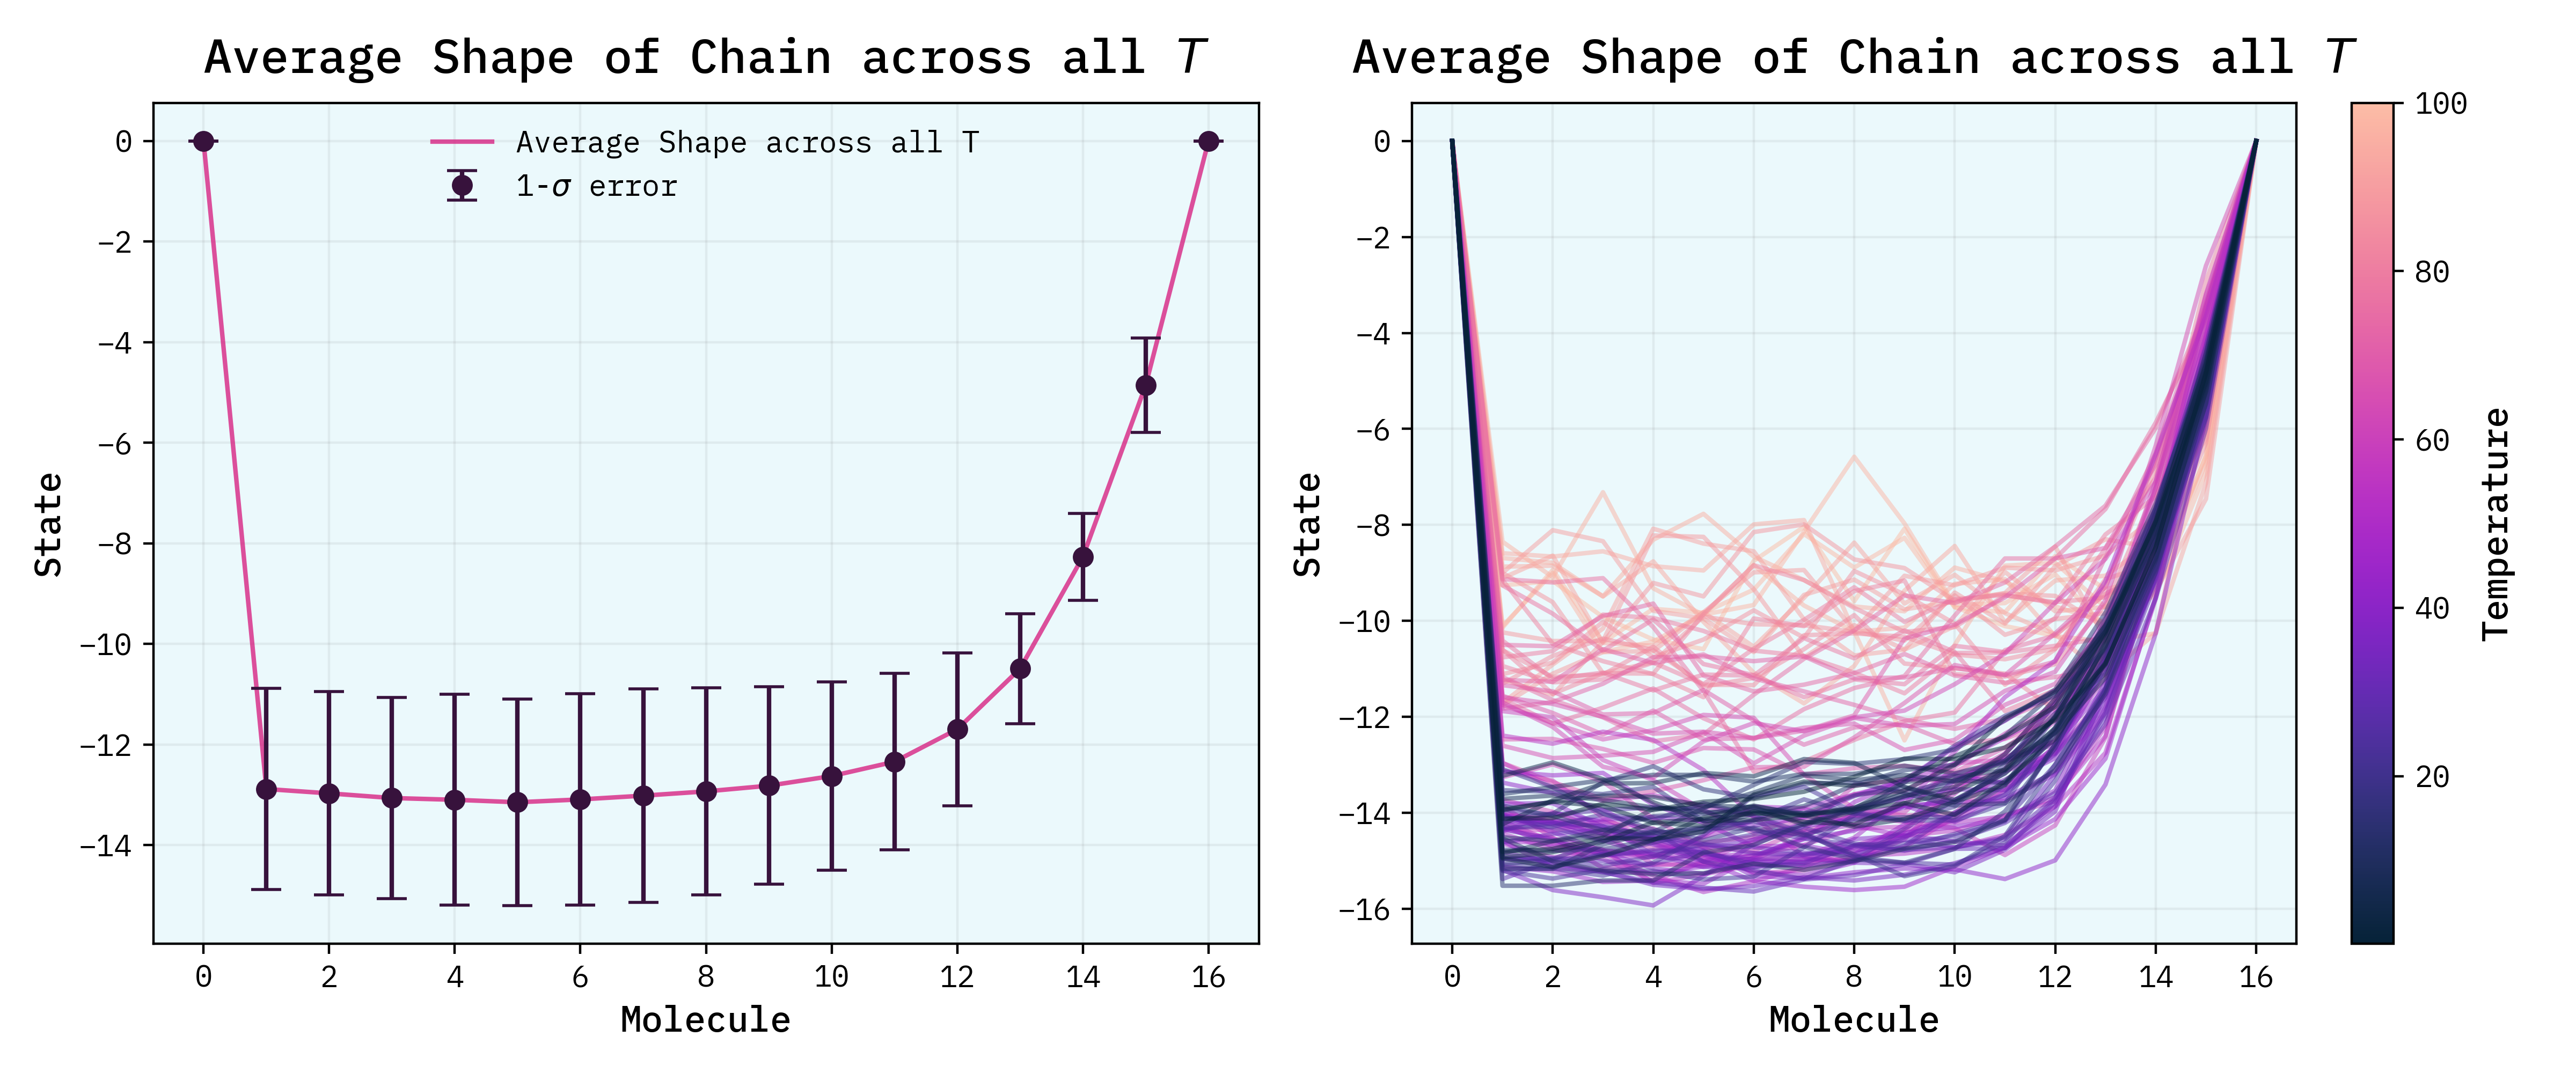
\includegraphics[width=.95\textwidth]{../MolecularChain2/Images/rand-init-T-spread.png}
    \caption{Average shape of the molecular chain across all temperatures and average shapes over repeat runs for each temperature.}
    \label{fig:molecular-chain-shapes}
\end{figure}


\section{Conclusion and Comments}

% Add references
% \newpage
\bibliographystyle{unsrt}
\bibliography{mod108}

% End document
\end{document}
